\typeout{************************************************}
\typeout{Chapter 9 Continuity: What It Isn't and What It Is}
\typeout{************************************************}
%
\begin{chapterptx}{Continuity: What It Isn't and What It Is}{}{Continuity: What It Isn't and What It Is}{}{}{x:chapter:Continuity}
	%
	%
	\typeout{************************************************}
	\typeout{Section 9.1 An Analytic Definition of Continuity}
	\typeout{************************************************}
	%
	\begin{sectionptx}{An Analytic Definition of Continuity}{}{An Analytic Definition of Continuity}{}{}{x:section:Continuity-AnalyticDef}
		Before the invention of calculus, the notion of continuity was treated intuitively if it was treated at all.  At first pass, it seems a very simple idea based solidly in our experience of the real world.  Standing on the bank we see a river flow past us continuously, not by tiny jerks.  Even when the flow might seem at first to be discontinuous, as when it drops precipitously over a cliff, a closer examination shows that it really is not. As the water approaches the cliff it speeds up.  When it finally goes over it accelerates very quickly but no matter how fast it goes it moves continuously, moving from here to there by occupying every point in between.  This is continuous motion. It never disappears over there and instantaneously reappears over here.  That would be discontinuous motion.%
		\par
		Similarly, a thrown stone flies continuously (and smoothly) from release point to landing point, passing through each point in its path.%
		\par
		But wait.%
		\par
		If the stone passes through discrete points it must be doing so by teeny tiny little jerks, mustn't it?  Otherwise how would it get from one point to the next?  Is it possible that motion in the real world, much like motion in a movie, is really composed of tiny jerks from one point to the next but that these tiny jerks are simply too small and too fast for our senses to detect?%
		\par
		If so, then the real world is more like the rational number line (\(\QQ\)) from \hyperref[x:chapter:NumbersRealRational]{Chapter~{\xreffont\ref{x:chapter:NumbersRealRational}}} than the real number line (\(\RR\)).  In that case, motion really consists of jumping discretely over the ``missing'' points (like \(\sqrt{2}\)) as we move from here to there. That may seem like a bizarre idea to you \textemdash{} it does to us as well \textemdash{} but the idea of continuous motion is equally bizarre.  It's just a little harder to see why.%
		\par
		The real world will be what it is regardless of what we believe it to be, but fortunately in mathematics we are \emph{not} constrained to live in it.  So we won't even try.  We will simply postulate that no such jerkiness exists; that all motion is continuous.%
		\par
		However we \emph{are} constrained to live with the logical consequences of our assumptions, once they are made.  These will lead us into some very deep waters indeed.%
		\par
		The intuitive treatment of continuity was maintained throughout the 1700's as it was not generally perceived that a truly rigorous definition was necessary.  Consider the following definition given by Euler in 1748.%
		\begin{quote}%
			A continuous curve is one such that its nature can be expressed by a single function of \(x.\) If a curve is of such a nature that for its various parts . . . different functions of \(x\) are required for its expression, . . . , then we call such a curve discontinuous.%
		\end{quote}
		However, the complexities associated with Fourier series and the types of functions that they represented caused mathematicians in the early \(1800\)s to rethink their notions of continuity.  As we saw in \hyperref[x:part:Interregnum]{Part~{\xreffont\ref{x:part:Interregnum}}}, the graph of the function defined by the Fourier series%
		\begin{equation*}
			\frac{4}{\pi}\sum_{k=0}^\infty\frac{\left(-1\right)^k}{\left(2k+1\right)} \cos \left(\left(2k+1\right)\pi x\right)
		\end{equation*}
		looked like this:%
		\begin{figureptx}{}{g:figure:idp167}{}%
			\begin{image}{0.125}{0.75}{0.125}%
				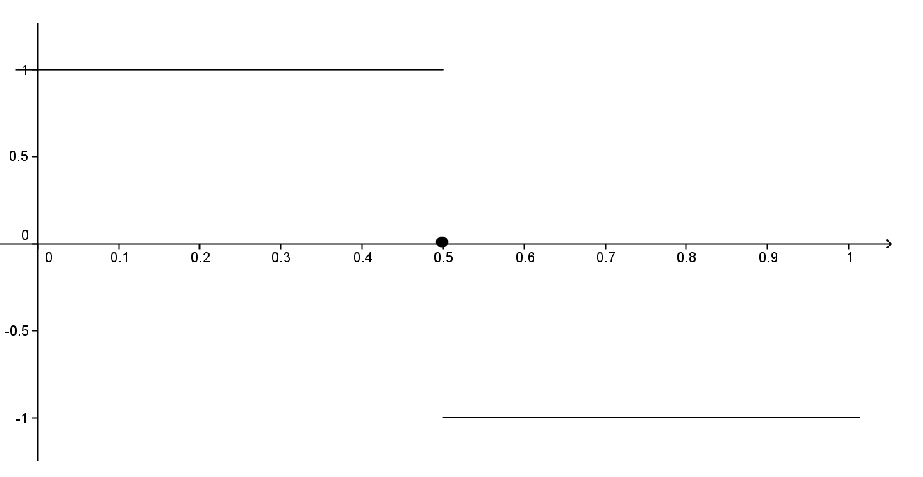
\includegraphics[width=\linewidth]{external/images/Ch5fig1.png}
			\end{image}%
			\tcblower
		\end{figureptx}%
		This function went against Euler's notion of what a continuous function should be.  Here, an infinite sum of continuous cosine curves provided a single expression which resulted in a ``discontinuous'' curve.  But as we've seen this didn't happen with power series and an intuitive notion of continuity is inadequate to explain the difference.  Even more perplexing is the following situation.  Intuitively, one would think that a continuous curve should have a tangent line at at least one point.  It may have a number of jagged points to it, but it should be ``smooth'' somewhere.  An example of this would be \(f(x)=x^{2/3}\).  Its graph is given by%
		\begin{figureptx}{}{g:figure:idp168}{}%
			\begin{image}{0.125}{0.75}{0.125}%
				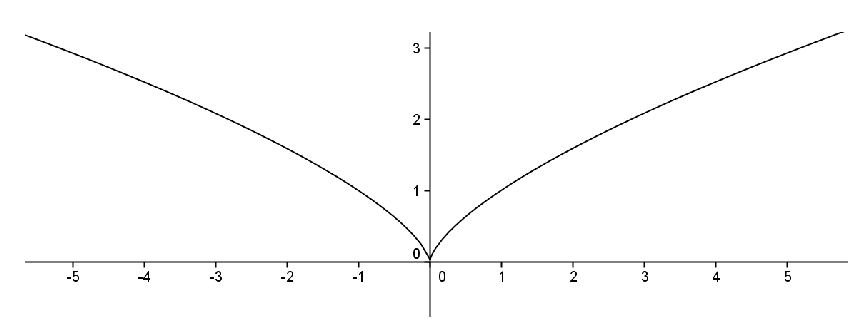
\includegraphics[width=\linewidth]{external/images/Ch5fig2.png}
			\end{image}%
			\tcblower
		\end{figureptx}%
		This function is not differentiable at the origin but it is differentiable everywhere else.  One could certainly come up with examples of functions which fail to be differentiable at any number of points but, intuitively, it would be reasonable%
		\begin{figureptx}{\href{https://mathshistory.st-andrews.ac.uk/Biographies/Weierstrass/}{Karl Weierstrass}\protect\footnotemark{}}{g:figure:idp169}{}%
			\index{Weierstrass, Karl!portrait of}%
			\begin{image}{0.325}{0.35}{0.325}%
				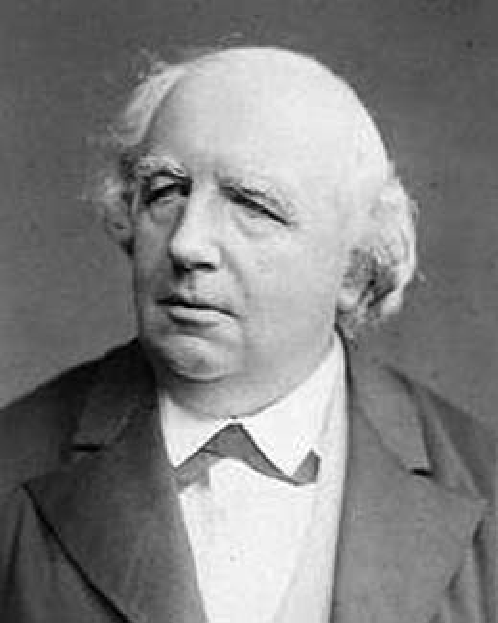
\includegraphics[width=\linewidth]{external/images/Weierstrass.png}
			\end{image}%
			\tcblower
		\end{figureptx}%
		\footnotetext[15]{\nolinkurl{mathshistory.st-andrews.ac.uk/Biographies/Weierstrass/}\label{g:fn:idp170}}%
		to expect that a continuous function should be differentiable \emph{somewhere}.  We might conjecture the following:%
		\begin{conjecture}{}{}{x:conjecture:conj_ContImplyDiff}%
			If \(f\) is continuous on an interval \(I\) then there is some \(a\in I\), such that \(f^\prime(a)\) exists.%
		\end{conjecture}
		Surprisingly, in \(1872\), Karl Weierstrass \index{Weierstrass, Karl} showed that the above conjecture is \alert{FALSE}. He did this by displaying the counterexample:%
		\begin{equation*}
			f(x)=\sum_{n=0}^\infty b^n\cos(a^n\pi x)\text{.}
		\end{equation*}
		%
		\par
		Weierstrass showed that if \(a\) is an odd integer, \(b\in(0,1)\), and \(ab>1+\frac{3}{2}\pi\), then \(f\) is continuous everywhere, but is nowhere differentiable.  Such a function is somewhat ``fractal'' in nature, and it is clear that a definition of continuity relying on intuition is inadequate to study it.%
		\begin{problem}{}{g:problem:idp171}%
			\begin{enumerate}[font=\bfseries,label=(\alph*),ref=\alph*]
				\item{}Given \(f(x)=\sum_{n=0}^\infty\left(\frac{1}{2}\right)^n\cos\left(a^n\pi
				x\right)\), what is the smallest value of \(a\) for which \(f\) satisfies Weierstrass' criterion to be continuous and nowhere differentiable.%
				\item{}Let \(f(x,N)=\sum_{n=0}^N\left(\frac{1}{2}\right)^n\cos\left(13^n\pi
				x\right)\) and use a computer algebra system to plot \(f(x,N)\) for \(N=0,1,2,3,4,10\) and \(x\in[0,1]\).%
				\item{}Plot \(f(x,10)\) for \(x\in[\,0,c]\), where \(c=0.1,0.01,0.001,0.0001,0.00001\).  Based upon what you see in parts b and c, why would we describe the function to be somewhat ``fractal'' in nature?%
			\end{enumerate}
		\end{problem}
		Just as it was important to define convergence with a rigorous definition without appealing to intuition or geometric representations, it is imperative that we define continuity in a rigorous fashion not relying on graphs.%
		\par
		The first appearance of a definition of continuity which did not rely on geometry or intuition was given in 1817 by Bernhard Bolzano \index{Bolzano, Bernhard} in a paper published in the Proceedings of the Prague Scientific Society entitled \textit{Rein analytischer Beweis des Lehrsatzes dass zwieschen je zwey Werthen, die ein entgegengesetztes Resultat gewaehren, wenigstens eine reele Wurzel der Gleichung liege} (Purely Analytic Proof of the Theorem that Between Any Two Values that Yield Results of Opposite Sign There Will be at Least One Real Root of the Equation).%
		\begin{figureptx}{\href{https://mathshistory.st-andrews.ac.uk/Biographies/Bolzano/}{Bernhard Bolzano}\protect\footnotemark{}}{g:figure:idp172}{}%
			\index{Bolzano, Bernhard!portrait of}%
			\begin{image}{0.325}{0.35}{0.325}%
				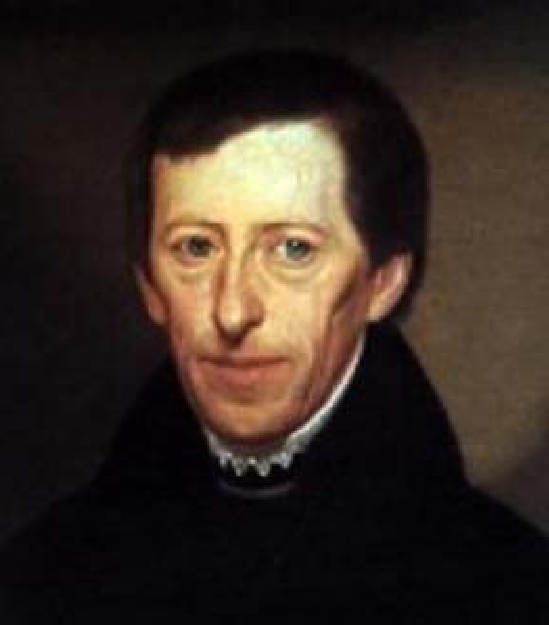
\includegraphics[width=\linewidth]{external/images/Bolzano.png}
			\end{image}%
			\tcblower
		\end{figureptx}%
		\footnotetext[16]{\nolinkurl{mathshistory.st-andrews.ac.uk/Biographies/Bolzano/}\label{g:fn:idp173}}%
		From the title it should be clear that in this paper Bolzano is proving the Intermediate Value Theorem.  To do this he needs a completely analytic definition of continuity.  The substance of Bolzano's idea is that if \(f\) is continuous at a point \(a\) then \(f(x)\) should be ``close to'' \(f(a)\) whenever \(x\) is ``close enough to'' \(a\).  More precisely, Bolzano said that \(f\) is continuous at \(a\) provided \(\abs{f(x)-f(a)}\) can be made smaller than any given quantity provided we make \(\abs{x-a}\) sufficiently small.%
		\par
		The language Bolzano uses is very similar to the language Leibniz \index{Leibniz, Gottfried Wilhelm} used when he postulated the existence of infinitesimally small numbers. Leibniz said that infinitesimals are ``smaller than any given quantity but not zero.'' Bolzano says that ``\(\abs{f(x)-f(a)}\) can be made smaller than any given quantity provided we make \(\abs{x-a}\) sufficiently small.'' But Bolzano stops short of saying that \(\abs{x-a}\) is \emph{infinitesimally} small.  Given \(a\), we can choose \(x\) so that \(\abs{x-a}\) is smaller than any real number we could name, say \(b\), provided we name \(b\) \emph{first}, but for any given choice of \(x\), \(\abs{x-a}\), and \(b\) are both still real numbers.  Possibly very small real numbers to be sure, but real numbers nonetheless.  Infinitesimals have no place in Bolzano's construction.%
		\par
		\index{Bolzano, Bernhard} Bolzano's paper was not well known when Cauchy \index{Cauchy, Augustin} proposed a similar definition in his \emph{Cours d'analyse}~\hyperlink{x:biblio:bradley09__cauch_cours}{[{\xreffont 1}]} of 1821 so it is usually Cauchy who is credited with this definition, but even Cauchy's definition is not quite tight enough for modern standards.  It was Karl Weierstrass in 1859 who finally gave the modern definition.%
		\begin{definition}{}{x:definition:def_continuity}%
			\index{continuity!definition of}\index{continuity} We say that a function \(\boldsymbol{f}\) is continuous at \(\boldsymbol{a}\) provided that for any \(\eps>0\), there exists a \(\delta>0\) such that if \(\abs{x-a}\lt
			\delta\) then \(|f(x)-f(a)|\lt \eps\).%
		\end{definition}
		Notice that the definition of continuity of a function is done point-by-point.  A function can certainly be continuous at some points while discontinuous at others.  When we say that \(f\) is continuous on an interval, then we mean that it is continuous at every point of that interval and, in theory, we would need to use the above definition to check continuity at each individual point.%
		\par
		\index{Extreme Value Theorem (EVT)!continuity and}\index{continuity!Extreme Value Theorem (EVT) and}\index{Intermediate Value Theorem (IVT)!continuity and}\index{continuity!Intermediate Value Theorem and} Our definition fits the bill in that it does not rely on either intuition or graphs, but it is this very non-intuitiveness that makes it hard to grasp.  It usually takes some time to become comfortable with this definition, let alone use it to prove theorems such as the Extreme Value Theorem and Intermediate Value Theorem.  So let's go slowly to develop a feel for it.%
		\par
		This definition spells out a completely black and white procedure: you give me a positive number \(\eps\), and I must be able to find a positive number \(\delta\) which satisfies a certain property.  If I can always do that then the function is continuous at the point of interest.%
		\par
		This definition also makes very precise what we mean when we say that \(f(x)\) should be ``close to'' \(f(a)\) whenever \(x\) is ``close enough to'' \(a\).  For example, intuitively we know that \(f(x)=x^2\) should be continuous at \(x=2\).  This means that we should be able to get \(x^2\) to within, say, \(\eps=.1\) of \(4\) provided we make \(x\) close enough to \(2\).  Specifically, we want \(3.9\lt x^2\lt 4.1\).  This happens exactly when \(\sqrt{3.9}\lt x\lt \sqrt{4.1}\).  Using the fact that \(\sqrt{3.9}\lt 1.98\) and \(2.02\lt \sqrt{4.1}\), then we can see that if we get \(x\) to within \(\delta=.02\) of \(2\), then \(\sqrt{3.9}\lt 1.98\lt x\lt 2.02\lt
		\sqrt{4.1}\) and so \(x^2\) will be within .\(1\) of \(\,4\).  This is very straightforward.  What makes this situation more difficult is that we must be able to do this for any \(\eps>0\).%
		\par
		Notice the similarity between this definition and the definition of convergence of a sequence.  Both definitions have the challenge of an \(\eps>0\).  In the definition of \(\lim_{n\rightarrow\infty}s_n=s\), we had to get \(s_n\) to within \(\eps\) of \(s\) by making \(n\) large enough.  For sequences, the challenge lies in making \(\abs{s_n-s}\) sufficiently small.  More precisely, given \(\eps>0\) we need to decide how large \(n\) should be to guarantee that \(\abs{s_n-s}\lt \eps\).%
		\par
		In our definition of continuity, we still need to make something small (namely \(\abs{f(x)-f(a)}\lt \eps\)), only this time, we need to determine how close \(x\) must be to \(a\) to ensure this will happen instead of determining how large \(n\) must be.%
		\par
		What makes \(f\) continuous at \(a\) is the arbitrary nature of \(\eps\) (as long as it is positive).  As \(\eps\) becomes smaller, this forces \(f(x)\) to be closer to \(f(a)\).  That we can always find a positive distance \(\delta\) to work is what we mean when we say that we can make \(f(x)\) as close to \(f(a)\) as we wish, provided we get \(x\) close enough to \(a\).  The sequence of pictures below illustrates that the phrase ``for any \(\eps>0\), there exists a \(\delta>0\) such that if \(|\,x-a|\lt \delta\) then \(|f(x)-f(a)|\lt \eps\)'' can be replaced by the equivalent formulation ``for any \(\eps>0\), there exists a \(\delta>0\) such that if \(a-\delta\lt x\lt a+\delta\) then \(f(a)-\eps\lt f(x)\lt
		f(a)+\eps\).'' This could also be replaced by the phrase ``for any \(\eps>0\), there exists a \(\delta>0\) such that if \(x\in(a-\delta,a+\delta)\) then \(f(x)\in(f(a)-\eps,f(a)+\eps)\).'' All of these equivalent formulations convey the idea that we can get \(f(x)\) to within \(\eps\) of \(f(a)\), provided we make \(x\) within \(\delta\) of \(a\), and we will use whichever formulation suits our needs in a particular application.%
		\begin{sidebyside}{2}{0.025}{0.025}{0.05}%
			\begin{sbspanel}{0.45}[center]%
				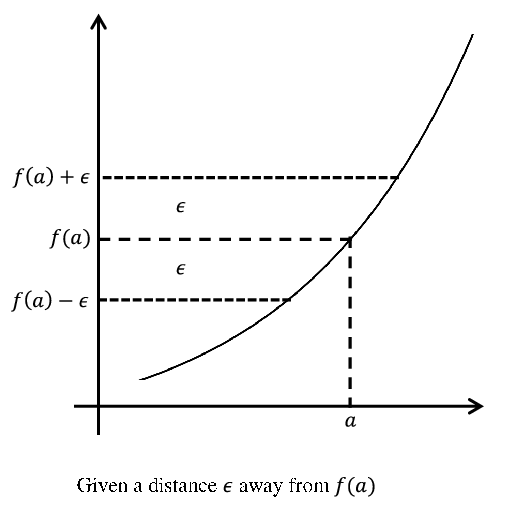
\includegraphics[width=\linewidth]{external/images/Ch5fig3a.png}
			\end{sbspanel}%
			\begin{sbspanel}{0.45}[center]%
				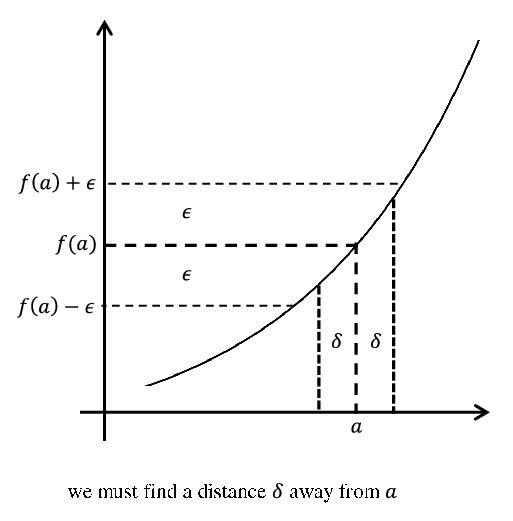
\includegraphics[width=\linewidth]{external/images/Ch5fig3b.png}
			\end{sbspanel}%
		\end{sidebyside}%
		\begin{sidebyside}{2}{0.025}{0.025}{0.05}%
			\begin{sbspanel}{0.45}[center]%
				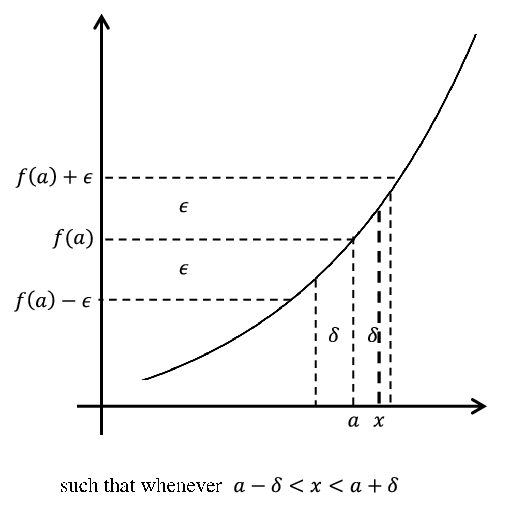
\includegraphics[width=\linewidth]{external/images/Ch5fig3c.png}
			\end{sbspanel}%
			\begin{sbspanel}{0.45}[center]%
				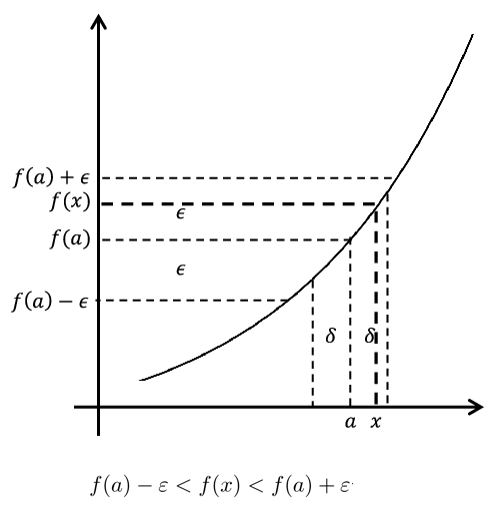
\includegraphics[width=\linewidth]{external/images/Ch5fig3d.png}
			\end{sbspanel}%
		\end{sidebyside}%
		The precision of the definition is what allows us to examine continuity without relying on pictures or vague notions such as ``nearness'' or ``getting closer to.'' We will now consider some examples to illustrate this precision.%
		\begin{example}{}{g:example:idp174}%
			Use the definition of continuity to show that \(f(x)=x\) is continuous at any point \(a\).%
		\end{example}
		If we were to draw the graph of this line, then you would likely say that this is obvious.  The point behind the definition is that we can back up your intuition in a rigorous manner.%
		\begin{proof}{}{g:proof:idp175}
			Let \(\eps>0\). Let \(\delta=\eps\). If \(|\,x-a|\lt \delta\), then%
			\begin{equation*}
				|f(x)-f(a)|=|\,x-a|\lt \eps
			\end{equation*}
			%
			\par
			Thus by the definition, \(f\) is continuous at \(a\).%
		\end{proof}
		\begin{problem}{}{g:problem:idp176}%
			\index{continuity!\(f(x) = mx +b\) is continuous everywhere} Use the definition of continuity to show that if \(m\) and \(b\) are fixed (but unspecified) real numbers then the function%
			\begin{equation*}
				f(x) = mx+b
			\end{equation*}
			is continuous at every real number \(a\).%
		\end{problem}
		\begin{example}{}{g:example:idp177}%
			Use the definition of continuity to show that \(f(x)=x^2\) is continuous at \(a=0\).%
		\end{example}
		\begin{proof}{}{g:proof:idp178}
			Let \(\eps>0\). Let \(\delta=\sqrt{\eps}\). If \(|\,x-0|\lt \delta\), then \(|\,x|\lt \sqrt{\eps}\). Thus%
			\begin{equation*}
				\abs{x^2-0^2}=|\,x|^2\lt \left(\sqrt{\eps}\right)^2=\eps\text{.}
			\end{equation*}
			%
			\par
			Thus by the definition, \(f\) is continuous at \(0\).%
		\end{proof}
		Notice that in these proofs, the challenge of an \(\eps>0\) was first given.  This is because the choice of \(\delta\) must depend upon \(\eps\).  Also notice that there was no explanation for our choice of \(\delta\).  We just supplied it and showed that it worked.  As long as \(\delta>0\), then this is all that is required.  In point of fact, the \(\delta\) we chose in each example was not the only choice that worked; any smaller \(\delta\) would work as well.%
		\begin{problem}{}{g:problem:idp179}%
			\begin{enumerate}[font=\bfseries,label=(\alph*),ref=\alph*]
				\item{}Given a particular \(\eps>0\) in the definition of continuity, show that if a particular \(\delta_0>0\) satisfies the definition, then any \(\delta\) with \(0\lt \delta\lt \delta_0\) will also work for this \(\eps\).%
				\item{}Show that if a \(\delta\) can be found to satisfy the conditions of the definition of continuity for a particular \(\eps_0>0\), then this \(\delta\) will also work for any \(\,\eps\) with \(0\lt \eps_0\lt
				\eps\).%
			\end{enumerate}
		\end{problem}
		It wasn't explicitly stated in the definition but when we say ``if \(\abs{x-a}\lt \delta\) then \(|f(x)-f(a)|\lt
		\eps\),'' we should be restricting ourselves to \(x\) values which are in the domain of the function \(f\), otherwise \(f(x)\) doesn't make sense.  We didn't put it in the definition because that definition was complicated enough without this technicality.  Also in the above examples, the functions were defined everywhere so this was a moot point.  We will continue with the convention that when we say ``if \(|\,x-a|\lt \delta\) then \(|f(x)-f(a)|\lt \eps\),'' we will be restricting ourselves to \(x\) values which are in the domain of the function \(f\).  This will allow us to examine continuity of functions not defined for all \(x\) without restating this restriction each time.%
		\begin{problem}{}{x:problem:prob_extended_sqrt_is_continuous_at_zero}%
			\index{continuity!\(\pm\sqrt{x}\) is continuous at zero} Use the definition of continuity to show that%
			\begin{equation*}
				f(x)= \begin{cases}\sqrt{x} \amp  \text{ if }  x\ge0\\ -\sqrt{-x} \amp  \text{ if }  x\lt 0 \end{cases}
			\end{equation*}
			is continuous at \(a=0\).%
		\end{problem}
		\begin{problem}{}{g:problem:idp180}%
			\index{\(\sqrt{x}\)!is continuous at zero} Use the definition of continuity to show that \(f(x)=
			\sqrt{x}\) is continuous at \(a=0\).  How is this problem different from \hyperref[x:problem:prob_extended_sqrt_is_continuous_at_zero]{problem~{\xreffont\ref{x:problem:prob_extended_sqrt_is_continuous_at_zero}}}? How is it similar?%
		\end{problem}
		Sometimes the \(\delta\) that will work for a particular \(\eps\) is fairly obvious to see, especially after you've gained some experience.  This is the case in the above examples (at least after looking back at the proofs).  However, the task of finding a \(\delta\) to work is usually not so obvious and requires some scrapwork.  This scrapwork is vital toward producing a \(\delta\), but again is not part of the polished proof.  This can be seen in the following example.%
		\begin{example}{}{x:example:example_SqrtContinuous}%
			Use the definition of continuity to prove that \(f(x)=\sqrt{x}\) is continuous at \(a=1\).%
			\par
			\terminology{SCRAPWORK}%
			\par
			As before, the scrapwork for these problems often consists of simply working backwards.  Specifically, given an \(\eps>0\), we need to find a \(\delta>0\) so that \(|\sqrt{x}-\sqrt{1}|\lt \eps\), whenever \(|\,x-1|\lt
			\delta\).  We work backwards from what we want, keeping an eye on the fact that we can control the size of \(\abs{x-1}\).%
			\begin{equation*}
				|\sqrt{x}-\sqrt{1}|=|\frac{\left(\sqrt{x}-1\right)\left(\sqrt{x}+1\right)}{\sqrt{x}+1}|=\frac{|\,x-1|}{\sqrt{x}+1}\lt |\,x-1|\text{.}
			\end{equation*}
			%
			\par
			This seems to suggest that we should make \(\delta=\eps\). We're now ready for the formal proof.%
		\end{example}
		\begin{proof}{}{g:proof:idp181}
			Let \(\eps>0\). Let \(\delta=\eps\). If \(|\,x-1|\lt \delta\), then \(|\,x-1|\lt \eps\), and so%
			\begin{equation*}
				\abs{\sqrt{x}-\sqrt{1}}=|\frac{\left(\sqrt{x}-1\right)\left(\sqrt{x}+1\right)}{ \sqrt{x}+1}|=\frac{|x-1|}{\sqrt{x}+1}\lt \abs{x-1}\lt \eps\text{.}
			\end{equation*}
			%
			\par
			Thus by definition, \(f(x)=\sqrt{x}\) is continuous at \(1\).%
		\end{proof}
		\begin{figureptx}{\href{https://mathshistory.st-andrews.ac.uk/Biographies/Halmos/}{Paul Halmos}\protect\footnotemark{}}{g:figure:idp182}{}%
			\index{Halmos, Paul!portrait of}%
			\begin{image}{0.325}{0.35}{0.325}%
				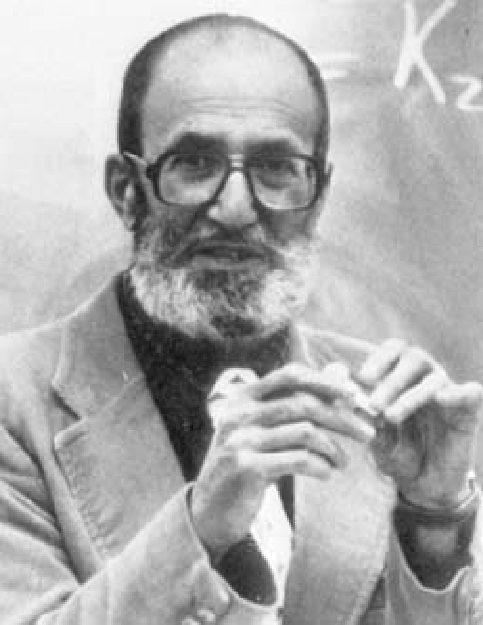
\includegraphics[width=\linewidth]{external/images/Halmos.png}
			\end{image}%
			\tcblower
		\end{figureptx}%
		\footnotetext[17]{\nolinkurl{mathshistory.st-andrews.ac.uk/Biographies/Halmos/}\label{g:fn:idp183}}%
		Bear in mind that someone reading the formal proof will not have seen the scrapwork, so the choice of \(\delta\) might seem rather mysterious.  However, you are in no way bound to motivate this choice of \(\delta\) and usually you should not, unless it is necessary for the formal proof.  All you have to do is find this \(\delta\) and show that it works.  Furthermore, to a trained reader, your ideas will come through when you demonstrate that your choice of \(\delta\) works.%
		\par
		Now reverse this last statement.  \emph{As} a trained reader, when you read the proof of a theorem it is \emph{your} responsibility to find the scrapwork, to see how the proof works and understand it fully.  As the renowned mathematical expositor Paul Halmos \index{Halmos, Paul} (1916-2006) said, ``Don't just read it; fight it! Ask your own questions, look for your own examples, discover your own proofs. Is the hypothesis necessary? Is the converse true? What happens in the classical special case? What about the degenerate cases? Where does the proof use the hypothesis?''%
		\par
		This is the way to learn mathematics.  It is really the only way.%
		\begin{problem}{}{g:problem:idp184}%
			Use the definition of continuity to show that \(f(x)=\sqrt{x}\) is continuous at any positive real number \(a\).%
		\end{problem}
		\begin{problem}{}{g:problem:idp185}%
			\begin{enumerate}[font=\bfseries,label=(\alph*),ref=\alph*]
				\item{}Use a unit circle to show that for \(0\leq\theta\lt
				\frac{\pi}{2}\), \(\sin \theta\leq\theta\) and \(1-\cos \theta\leq\theta\) and conclude \(\abs{\sin
					\theta}\leq\abs{\theta}\) and \(\abs{1-\cos
					\theta}\leq\abs{\theta}\) for \(-\frac{\pi}{2}\lt
				\theta\) \(\lt \frac{\pi}{2}\).%
				\item{}Use the definition of continuity to prove that \(f(x)=\sin x\) is continuous at any point \(a\).%
				\par\smallskip%
				\noindent\textbf{\blocktitlefont Hint}.\hypertarget{g:hint:idp186}{}\quad{}\(\sin x=\sin\left(x-a+a\right)\).%
			\end{enumerate}
		\end{problem}
		\begin{problem}{}{g:problem:idp187}%
			\begin{enumerate}[font=\bfseries,label=(\alph*),ref=\alph*]
				\item{}Use the definition of continuity to show that \(f(x)=e^x\) is continuous at \(a=0\).%
				\item{}Show that \(f(x)=e^x\) is continuous at any point \(a\).%
				\par\smallskip%
				\noindent\textbf{\blocktitlefont Hint}.\hypertarget{g:hint:idp188}{}\quad{}Rewrite \(e^x-e^a\) as \(e^{a+(x-a)}-e^a\) and use what you proved in part a.%
			\end{enumerate}
		\end{problem}
		In the above problems, we used the definition of continuity to verify our intuition about the continuity of familiar functions.  The advantage of this analytic definition is that it can be applied when the function is not so intuitive.  Consider, for example, the function given at the end of the last chapter.%
		\begin{equation*}
			f(x)= \begin{cases}
				x\,\sin\left(\frac{1}{x}\right),\amp \text{ if } x\neq 0\\
				0, \amp \text{ if } x=0 
			\end{cases}  \text{.}
		\end{equation*}
		%
		\par
		Near zero, the graph of \(f(x)\) looks like this:%
		\begin{image}{0.125}{0.75}{0.125}%
			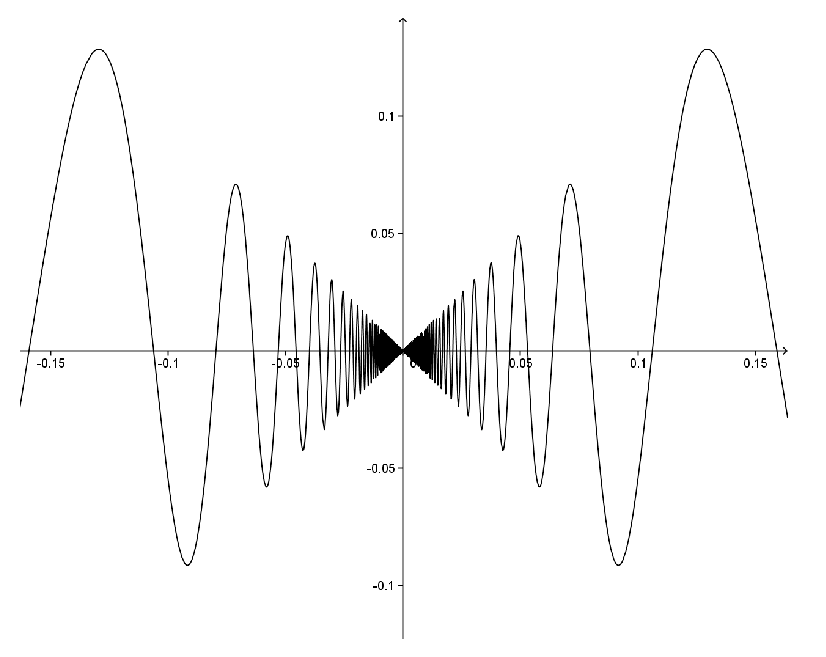
\includegraphics[width=\linewidth]{external/images/Ch5fig4.png}
		\end{image}%
		As we mentioned in the previous chapter, since sin\(\left(\frac{1}{x}\right)\) oscillates infinitely often as \(x\) nears zero this graph must be viewed with a certain amount of suspicion.  However our completely analytic definition of continuity shows that this function is, in fact, continuous at 0.%
		\begin{problem}{The Topologist's Sine Function.}{g:problem:idp189}%
			\index{Topologist's sine function!is continuous at zero} Use the definition of continuity to show that%
			\begin{equation*}
				f(x)= \begin{cases}x\,\sin\left(\frac{1}{x}\right),\amp \text{ if } x\neq 0\\ 0\text{,} \amp \text{ if } x=0 \end{cases}
			\end{equation*}
			is continuous at \(0\).%
		\end{problem}
		Even more perplexing is the function defined by%
		\begin{equation*}
			D(x)= \begin{cases}
				x, \amp \text{ if } x\text{ is rational } \\
				0, \amp \text{ if } x\text{ is irrational } . 
			\end{cases} 
		\end{equation*}
		%
		\par
		To the naked eye, the graph of this function looks like the lines \(y=0\) and \(y=x\).  Of course, such a graph would not be the graph of a function.  Actually, both of these lines have holes in them.  Wherever there is a point on one line there is a ``hole'' on the other.  Each of these holes are the width of a single point (that is, their ``width'' is zero!) so they are invisible to the naked eye (or even magnified under the most powerful microscope available).  This idea is illustrated in the following graph%
		\begin{image}{0.2}{0.6}{0.2}%
			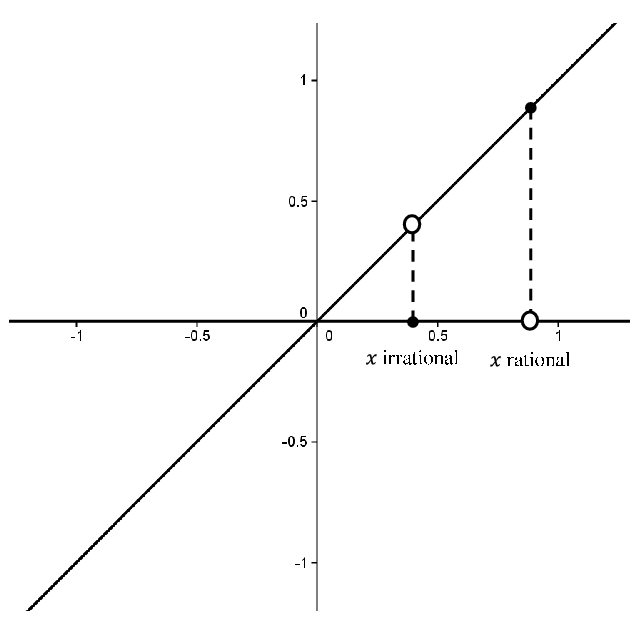
\includegraphics[width=\linewidth]{external/images/Ch5fig5.png}
		\end{image}%
		Can such a function so ``full of holes'' actually be continuous anywhere?  It turns out that we can use our definition to show that this function is, in fact, continuous at \(0\) and at no other point.%
		\begin{problem}{}{g:problem:idp190}%
			\begin{enumerate}[font=\bfseries,label=(\alph*),ref=\alph*]
				\item{}Use the definition of continuity to show that the function%
				\begin{equation*}
					D(x)= \begin{cases}
						x,\amp \text{ if } x\text{ is rational } \\
						0,\amp \text{ if } x\text{ is irrational } \end{cases} 
				\end{equation*}
				is continuous at \(0\).%
				\item{}Let \(a\neq 0\).  Use the definition of continuity to show that \(D\) is not continuous at \(a\).%
				\par\smallskip%
				\noindent\textbf{\blocktitlefont Hint}.\hypertarget{g:hint:idp191}{}\quad{}You might want to break this up into two cases where \(a\) is rational or irrational.  Show that no choice of \(\delta>0\) will work for \(\eps=|\,a|\).  Note that \hyperref[x:theorem:thm_IrrationalBetweenIrrationals]{Theorem~{\xreffont\ref{x:theorem:thm_IrrationalBetweenIrrationals}}} of \hyperref[x:chapter:NumbersRealRational]{Chapter~{\xreffont\ref{x:chapter:NumbersRealRational}}} will probably help here.%
			\end{enumerate}
		\end{problem}
	\end{sectionptx}
	%
	%
	\typeout{************************************************}
	\typeout{Section 9.2 Sequences and Continuity}
	\typeout{************************************************}
	%
	\begin{sectionptx}{Sequences and Continuity}{}{Sequences and Continuity}{}{}{x:section:SequencesAndContinuity}
		There is an alternative way to prove that the function%
		\begin{equation*}
			D(x)=\left\{ \begin{matrix}x\text{,} \amp \text{ if } x\text{ is rational } \\ 0\text{,} \amp \text{ if } x\text{ is irrational } \end{matrix} \right.
		\end{equation*}
		is not continuous at \(a\neq 0\).  We will examine this by looking at the relationship between our definitions of convergence and continuity.  The two ideas are actually quite closely connected, as illustrated by the following very useful theorem.%
		\begin{theorem}{}{}{x:theorem:thm_LimDefOfContinuity}%
			\index{continuity!via limits} The function \(f\) is continuous at \(a\) if and only if \(f\) satisfies the following property:%
			\begin{equation*}
				\forall\text{ sequences } \left(x_n\right)\text{, if } \,\,\lim_{n\rightarrow\infty}x_n=a \text{ then} \lim_{n\rightarrow\infty}f(x_n)=f(a).{}
			\end{equation*}
			%
		\end{theorem}
		\hyperref[x:theorem:thm_LimDefOfContinuity]{Theorem~{\xreffont\ref{x:theorem:thm_LimDefOfContinuity}}} says that in order for \(f\) to be continuous, it is necessary and sufficient that any sequence \(\left(x_n\right)\) converging to \(a\) must force the sequence \(\left(f(x_n)\right)\) to converge to \(f(a)\).  A picture of this situation is below though, as always, the formal proof will not rely on the diagram.%
		\begin{image}{0.315}{0.37}{0.315}%
			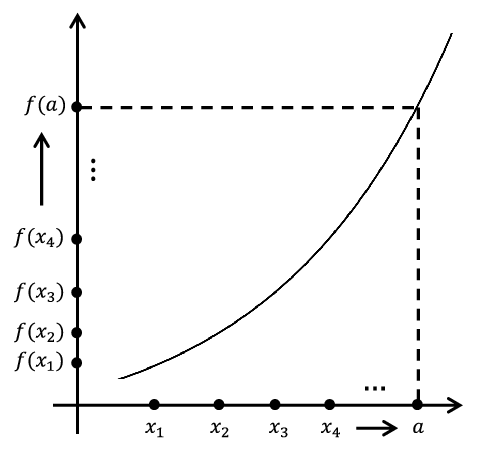
\includegraphics[width=\linewidth]{external/images/Ch5fig6.png}
		\end{image}%
		This theorem is especially useful for showing that a function \(f,\) is not continuous at a point \(a\); all we need to do is exhibit a sequence \(\left(x_n\right)\) converging to \(a\) such that the sequence \(\lim_{n\rightarrow\infty}f(x_n)\) does \emph{not} converge to \(f(a)\).  Let's demonstrate this idea before we tackle the proof of \hyperref[x:theorem:thm_LimDefOfContinuity]{Theorem~{\xreffont\ref{x:theorem:thm_LimDefOfContinuity}}}.%
		\begin{example}{}{x:example:example_HeavisideNotContinuous}%
			Use \hyperref[x:theorem:thm_LimDefOfContinuity]{Theorem~{\xreffont\ref{x:theorem:thm_LimDefOfContinuity}}} to prove that%
			\begin{equation*}
				f(x)= \begin{cases}\frac{|x|}{x}\text{,} \amp \text{ if } x\neq 0\\ 0\text{,} \amp \text{ if } x=0 \end{cases}
			\end{equation*}
			is not continuous at \(0\).%
		\end{example}
		\begin{proof}{}{g:proof:idp192}
			First notice that \(f\) can be written as%
			\begin{equation*}
				f(x)= \begin{cases}1\amp \text{ if } x>0\\ -1\amp \text{ if } x\lt 0\\ 0\amp \text{ if } x=0 \end{cases} \text{.}
			\end{equation*}
			%
			\par
			To show that \(f\) is not continuous at \(0\), all we need to do is create a single sequence \(\left(x_n\right)\)which converges to \(0\), but for which the sequence \(\left(f\left(x_n\right)\right)\) does not converge to \(f(0)=0\).  For a function like this one, just about any sequence will do, but let's use \(\left(\frac{1}{n}\right)\), just because it is an old familiar friend.%
			\par
			We have \(\displaystyle\lim_{n\rightarrow\infty}\frac{1}{n}=0\), but \(\displaystyle\lim_{n\rightarrow\infty}f\left(\frac{1}{n}\right)=\lim_{n\rightarrow
				\infty}1=1\neq 0=f(0)\).  Thus by \hyperref[x:theorem:thm_LimDefOfContinuity]{Theorem~{\xreffont\ref{x:theorem:thm_LimDefOfContinuity}}}, \(f\) is not continuous at \(0\).%
		\end{proof}
		\begin{problem}{}{g:problem:idp193}%
			\index{continuity!Heaviside's function is not continuous at zero} Use \hyperref[x:theorem:thm_LimDefOfContinuity]{Theorem~{\xreffont\ref{x:theorem:thm_LimDefOfContinuity}}} to show that%
			\begin{equation*}
				f(x)= \begin{cases}
					\frac{\abs{x}}{x},\amp \text{ if } x\neq 0\\
					a, \amp \text{ if } x=0 \end{cases}  
			\end{equation*}
			is not continuous at \(0\), no matter what value \(a\) is.%
		\end{problem}
		\begin{problem}{}{g:problem:idp194}%
			Use \hyperref[x:theorem:thm_LimDefOfContinuity]{Theorem~{\xreffont\ref{x:theorem:thm_LimDefOfContinuity}}} to show that%
			\begin{equation*}
				D(x)= \begin{cases}
					x, \amp \text{ if } x\text{ is rational } \\
					0, \amp \text{ if } x\text{ is irrational } \end{cases}  
			\end{equation*}
			is not continuous at \(a\neq 0\).%
		\end{problem}
		\begin{problem}{}{g:problem:idp195}%
			The function \(T(x)=\sin\left(\frac{1}{x}\right)\) is often called the topologist's sine curve.  Whereas \(\sin
			x\) has roots at \(n\pi\), \(n\in\ZZ\) and oscillates infinitely often as \(x\rightarrow\pm\infty\), \(T\) has roots at \(\frac{1}{n\pi},\,n\in\ZZ,\,n\neq
			0\), and oscillates infinitely often as \(x\) approaches zero.  A rendition of the graph follows.%
			\begin{image}{0.125}{0.75}{0.125}%
				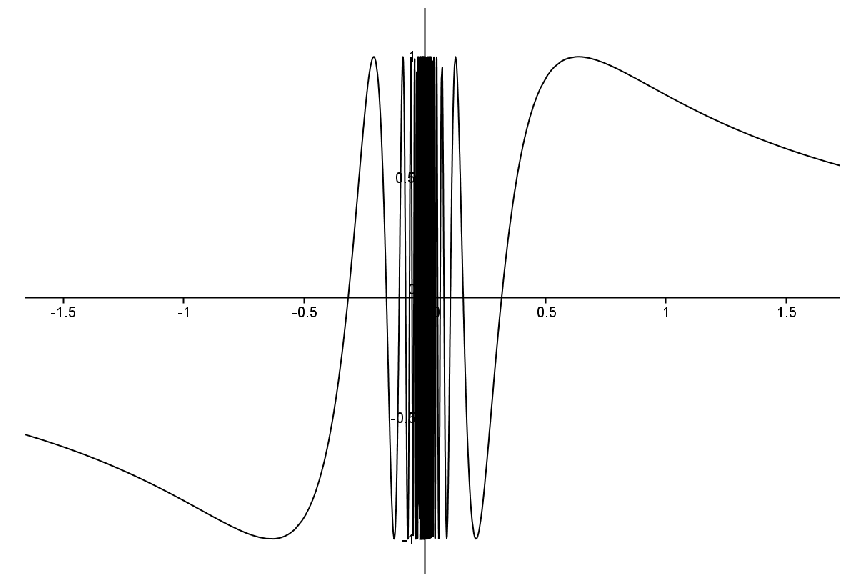
\includegraphics[width=\linewidth]{external/images/Ch5fig7.png}
			\end{image}%
			Notice that \(T\) is not even defined at \(x=0\). We can extend \(T\) to be defined at 0 by simply choosing a value for \(T(0):\)%
			\begin{equation*}
				T(x)= \begin{cases}
					\sin\left(\frac{1}{x}\right),\amp \text{ if } x\neq 0\\ 
					b,\amp \text{ if } x=0 \end{cases} \text{.}
			\end{equation*}
			%
			\par
			Use \hyperref[x:theorem:thm_LimDefOfContinuity]{Theorem~{\xreffont\ref{x:theorem:thm_LimDefOfContinuity}}} to show that \(T\) is not continuous at \(0\), no matter what value is chosen for \(b\).%
		\end{problem}
		\begin{proof}{Sketch of the Proof of Theorem~{\xreffont\ref*{x:theorem:thm_LimDefOfContinuity}}.}{g:proof:idp196}
			We've seen how we can use \hyperref[x:theorem:thm_LimDefOfContinuity]{Theorem~{\xreffont\ref{x:theorem:thm_LimDefOfContinuity}}}, now we need to prove \hyperref[x:theorem:thm_LimDefOfContinuity]{Theorem~{\xreffont\ref{x:theorem:thm_LimDefOfContinuity}}}.  The forward direction is fairly straightforward.  So we assume that \(f\) is continuous at \(a\) and start with a sequence \(\left(x_n\right)\) which converges to \(a\). What is left to show is that \(\lim_{n\rightarrow\infty}f(x_n)=f(a)\).  If you write down the definitions of \(f\) being continuous at \(a\), \(\lim_{n\rightarrow\infty}x_n=a\), and \(\lim_{n\rightarrow\infty}f(x_n)=f(a)\), you should be able to get from what you are assuming to what you want to conclude.%
			\par
			To prove the converse, it is convenient to prove its contrapositive.  That is, we want to prove that if \(f\) is not continuous at \(a\) then we can construct a sequence \(\left(x_n\right)\) that converges to \(a\) but \(\left(f(x_n)\right)\)does not converge to \(f(a)\). First we need to recognize what it means for \(f\) to not be continuous at \(a\).  This says that somewhere there exists an \(\eps>0\), such that no choice of \(\delta>0\) will work for this.  That is, for any such \(\delta\), there will exist \(x\), such that \(|\,x-a|\lt \delta\), but \(|f(x)-f(a)|\geq\eps\). With this in mind, if \(\delta=1\), then there will exist an \(x_1\) such that \(|\,x_1-a|\lt 1\), but \(|f(x_1)-f(a)|\geq\eps\).  Similarly, if \(\delta=\frac{1}{2}\), then there will exist an \(x_2\) such that \(|\,x_2-a|\lt \frac{1}{2}\), but \(|\,f(x_2)-f(a)|\geq\eps\).  If we continue in this fashion, we will create a sequence \(\left(x_n\right)\) such that \(|\,x_n-a|\lt \frac{1}{n}\), but \(|f(x_n)-f(a)|\geq\eps\).  This should do the trick.%
		\end{proof}
		\begin{problem}{}{g:problem:idp197}%
			\index{continuity!via limits}\index{limit!\(\limit{x}{a}{f(x)}=f(a)\) implies \(f(x)\) is continuous} Turn the ideas of the previous two paragraphs into a formal proof of \hyperref[x:theorem:thm_LimDefOfContinuity]{Theorem~{\xreffont\ref{x:theorem:thm_LimDefOfContinuity}}}.%
		\end{problem}
		\hyperref[x:theorem:thm_LimDefOfContinuity]{Theorem~{\xreffont\ref{x:theorem:thm_LimDefOfContinuity}}} is a very useful result. It is a bridge between the ideas of convergence and continuity so it allows us to bring all of the theory we developed in \hyperref[x:chapter:Convergence]{Chapter~{\xreffont\ref{x:chapter:Convergence}}} to bear on continuity questions. For example consider the following.%
		\begin{theorem}{}{}{x:theorem:thm_ContSumProd}%
			\index{continuous functions!sum of continuous functions is continuous} Suppose \(f\) and \(g\) are both continuous at \(a\). Then \(f+g\) and \(f\cdot g\) are continuous at \(a\).%
		\end{theorem}
		\begin{proof}{}{g:proof:idp198}
			We could use the definition of continuity to prove \hyperref[x:theorem:thm_ContSumProd]{Theorem~{\xreffont\ref{x:theorem:thm_ContSumProd}}}, but \hyperref[x:theorem:thm_LimDefOfContinuity]{Theorem~{\xreffont\ref{x:theorem:thm_LimDefOfContinuity}}} makes our job much easier.  For example, to show that \(f+g\) is continuous, consider any sequence \(\left(x_n\right)\) which converges to \(a\).  Since \(f\) is continuous at \(a\), then by \hyperref[x:theorem:thm_LimDefOfContinuity]{Theorem~{\xreffont\ref{x:theorem:thm_LimDefOfContinuity}}}, \(\lim_{n\rightarrow\infty}f(x_n)=f(a)\).  Likewise, since \(g\) is continuous at \(a\), then \(\lim_{n\rightarrow\infty}g(x_n)=g(a)\).%
			\par
			By \hyperref[x:theorem:thm_SumOfSequences]{Theorem~{\xreffont\ref{x:theorem:thm_SumOfSequences}}} of \hyperref[x:chapter:Convergence]{Chapter~{\xreffont\ref{x:chapter:Convergence}}},\(\)%
			\begin{alignat*}{1}
				\lim_{n\rightarrow\infty}(f+g)(x_n)\amp=\lim_{n\rightarrow\infty} \left(f(x_n)+g(x_n)\right)\\
				\amp =\lim_{n\rightarrow\infty}f(x_n)+\,\lim_{n \rightarrow\infty}g(x_n)\\
				\amp =f(a)+g(a)\\
				\amp =(f+g)(a)\text{.}
			\end{alignat*}
			Thus by \hyperref[x:theorem:thm_LimDefOfContinuity]{Theorem~{\xreffont\ref{x:theorem:thm_LimDefOfContinuity}}}, \(f+g\) is continuous at \(a\).  The proof that \(f\cdot g\) is continuous at \(a\) is similar.%
		\end{proof}
		\begin{problem}{}{g:problem:idp199}%
			Use \hyperref[x:theorem:thm_LimDefOfContinuity]{Theorem~{\xreffont\ref{x:theorem:thm_LimDefOfContinuity}}} to show that if \(f\) and \(g\) are continuous at \(a\), then \(f\cdot g\) is continuous at \(a\).%
		\end{problem}
		By employing \hyperref[x:theorem:thm_ContSumProd]{Theorem~{\xreffont\ref{x:theorem:thm_ContSumProd}}} a finite number of times, we can see that a finite sum of continuous functions is continuous. That is, if \(f_1,\,f_2,\,\ldots,\,f_n\) are all continuous at \(a\) then \(\sum_{j=1}^nf_j\) is continuous at \(a\). But what about an infinite sum? Specifically, suppose \(f_1,\,f_2,f_3,\ldots\) are all continuous at \(a\). Consider the following argument.%
		\par
		Let \(\eps>0\). Since \(f_j\) is continuous at \(a\), then there exists \(\delta_j>0\) such that if \(|\,x-a|\lt \delta_j\), then \(|f_j(x)-f_j(a)|\lt \frac{\eps}{2^j}\). Let \(\delta=\)min\(\left(\delta_1,\,\delta_2,\,\ldots\right)\). If \(|\,x-a|\lt \delta\), then%
		\begin{equation*}
			\left|\sum_{j=1}^\infty f_j(x)-\sum_{j=1}^\infty f_j(a)\right|=\left|\sum_{j=1}^\infty\left(f_j(x)-f_j(a)\right)\right|
		\end{equation*}
		%
		\begin{equation*}
			\leq\,\sum_{j=1}^\infty|f_j(x)-f_j(a)|\lt \sum_{j=1}^\infty\frac{ \eps}{2^j}=\eps\text{.}
		\end{equation*}
		%
		\par
		Thus by definition, \(\sum_{j=1}^\infty f_j\) is continuous at \(a\).%
		\par
		This argument seems to say that an infinite sum of continuous functions must be continuous (provided it converges). However we know that the Fourier series%
		\begin{equation*}
			\frac{4}{\pi}\sum_{k=0}^\infty\frac{\left(-1\right)^k}{\left(2k+1\right)}\cos\left(\left(2k+1\right)\pi x\right)
		\end{equation*}
		is a counterexample to this, as it is an infinite sum of continuous functions which does not converge to a continuous function. Something fundamental seems to have gone wrong here. Can you tell what it is?%
		\par
		This is a question we will spend considerable time addressing in \hyperref[x:chapter:PowerSeriesRedux]{Chapter~{\xreffont\ref{x:chapter:PowerSeriesRedux}}} (in particular, see \hyperref[x:problem:prob_Cauchy_s_incorrect_proof]{problem~{\xreffont\ref{x:problem:prob_Cauchy_s_incorrect_proof}}}) so if you don't see the difficulty, don't worry; you will. In the meantime keep this problem tucked away in your consciousness. It is, as we said, fundamental.%
		\par
		\hyperref[x:theorem:thm_LimDefOfContinuity]{Theorem~{\xreffont\ref{x:theorem:thm_LimDefOfContinuity}}} will also handle quotients of continuous functions. There is however a small detail that needs to be addressed first. Obviously, when we consider the continuity of \(f/g\) at \(a\),\(\)we need to assume that \(g(a)\neq 0\). However, \(g\) may be zero at other values. How do we know that when we choose our sequence \(\left(x_n\right)\) converging to \(a\) that \(g(x_n)\) is not zero? This would mess up our idea of using the corresponding theorem for sequences (\hyperref[x:theorem:thm_LimitOfQuotient]{Theorem~{\xreffont\ref{x:theorem:thm_LimitOfQuotient}}} from \hyperref[x:chapter:Convergence]{Chapter~{\xreffont\ref{x:chapter:Convergence}}}). This can be handled with the following lemma.%
		\begin{lemma}{}{}{x:lemma:lem_BoundedAwayFromZero}%
			If \(g\) is continuous at \(a\) and \(g(a)\neq 0\), then there exists \(\delta>0\) such that \(g(x)\neq 0\) for all \(x\in(a-\delta,a+\delta)\).%
		\end{lemma}
		\begin{problem}{}{g:problem:idp200}%
			Prove \hyperref[x:lemma:lem_BoundedAwayFromZero]{Lemma~{\xreffont\ref{x:lemma:lem_BoundedAwayFromZero}}}.%
			\par\smallskip%
			\noindent\textbf{\blocktitlefont Hint}.\hypertarget{g:hint:idp201}{}\quad{}Consider the case where \(g(a)>0\). Use the definition with \(\eps=\frac{g(a)}{2}\). The picture is below; make it formal.%
			\begin{image}{0.125}{0.75}{0.125}%
				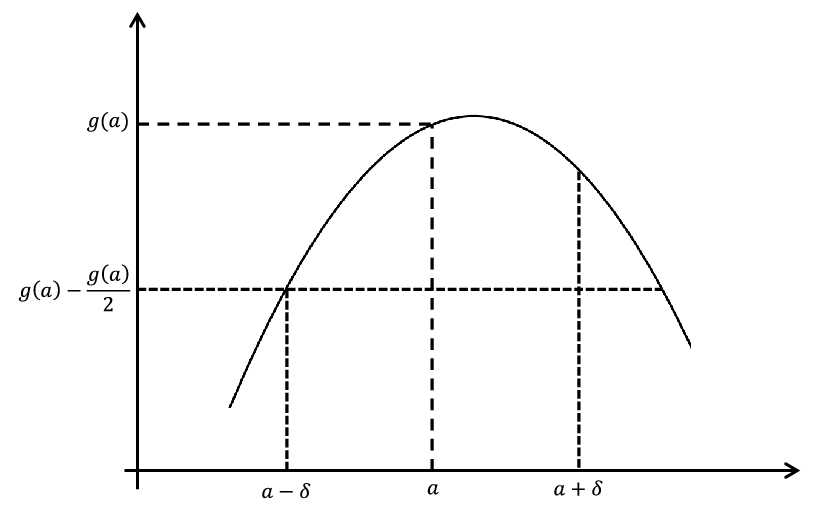
\includegraphics[width=\linewidth]{external/images/Ch5fig8.png}
			\end{image}%
			For the case \(g(a)\lt 0\), consider the function \(-g\).%
		\end{problem}
		A consequence of this lemma is that if we start with a sequence \(\left(x_n\right)\) converging to \(a\), then for \(n\) sufficiently large, \(g(x_n)\neq 0\).%
		\begin{problem}{}{g:problem:idp202}%
			Use \hyperref[x:theorem:thm_LimDefOfContinuity]{Theorem~{\xreffont\ref{x:theorem:thm_LimDefOfContinuity}}}, to prove that if \(f\) and \(g\) are continuous at \(a\) and \(g(a)\neq 0\), then \(f/g\) is continuous at \(a\).%
		\end{problem}
		\begin{theorem}{}{}{x:theorem:thm_ContComp}%
			\index{continuous functions!the composition of continuous functions is continuous}%
			Suppose \(f\) is continuous at \(a\) and \(g\) is continuous at \(f(a)\).  Then \(g\circ f\) is continuous at \(a.\) (Note that \((g\circ f)(x)=g(f(x))\).)%
		\end{theorem}
		\begin{problem}{}{g:problem:idp203}%
			Prove \hyperref[x:theorem:thm_ContComp]{Theorem~{\xreffont\ref{x:theorem:thm_ContComp}}}%
			\begin{enumerate}[font=\bfseries,label=(\alph*),ref=\alph*]
				\item{}Using the definition of continuity.%
				\item{}Using \hyperref[x:theorem:thm_LimDefOfContinuity]{Theorem~{\xreffont\ref{x:theorem:thm_LimDefOfContinuity}}}.%
			\end{enumerate}
		\end{problem}
		The above theorems allow us to build continuous functions from other continuous functions.  For example, knowing that \(f(x)=x\) and \(g(x)=c\) are continuous, we can conclude that any polynomial,%
		\begin{equation*}
			p(x)=a_nx^n+a_{n-1}x^{n-1}+\cdots+a_1x+a_0
		\end{equation*}
		is continuous as well. We also know that functions such as \(f(x)=\sin\left(e^x\right)\) are continuous without having to rely on the definition.%
		\begin{problem}{}{g:problem:idp204}%
			Show that each of the following is a continuous function at every point in its domain.%
			\begin{enumerate}[font=\bfseries,label=(\alph*),ref=\alph*]
				\item{}Any polynomial.%
				\item{}Any rational function. (A rational function is defined to be a ratio of polynomials.)%
				\item{}\(\cos x\).%
				\item{}The other trig functions: \(\tan(x)\), \(\cot(x)\), \(\sec(x)\), and \(\csc(x)\).%
			\end{enumerate}
		\end{problem}
		\begin{problem}{}{g:problem:idp205}%
			What allows us to conclude that \(f(x)=\sin\left(e^x\right)\) is continuous at any point \(a\) without referring back to the definition of continuity?%
		\end{problem}
		\hyperref[x:theorem:thm_LimDefOfContinuity]{Theorem~{\xreffont\ref{x:theorem:thm_LimDefOfContinuity}}} can also be used to study the convergence of sequences.  For example, since \(f(x)=e^x\) is continuous at any point and \(\lim_{n\rightarrow\infty}\frac{n+1}{n}=1\), then \(\lim_{n\rightarrow\infty}e^{\left(\frac{n+1}{n}\right)}=e\). This also illustrates a certain way of thinking about continuous functions.  They are the ones where we can ``commute'' the function and a limit of a sequence.  Specifically, if \(f\) is continuous at \(a\) and \(\lim_{n\rightarrow\infty}x_n=a\), then \(\lim_{n\rightarrow\infty}f(x_n)=f(a)=f\left(\lim_{n\rightarrow\infty}x_n\right)\).%
		\begin{problem}{}{g:problem:idp206}%
			Compute the following limits. Be sure to point out how continuity is involved.%
			\begin{enumerate}[font=\bfseries,label=(\alph*),ref=\alph*]
				\item{}\(\displaystyle\lim_{n\rightarrow\infty}\sin\left(\frac{n\pi}{2n+1}\right)\)%
				\item{}\(\displaystyle\lim_{n\rightarrow\infty}\sqrt{\frac{n}{n^2+1}}\)%
				\item{}\(\displaystyle\lim_{n\rightarrow\infty}e^{\left(\text{ sin } \left(1/n\right)\right)}\)%
			\end{enumerate}
		\end{problem}
		Having this rigorous formulation of continuity is necessary for proving the Extreme Value Theorem and the Mean Value Theorem. However there is one more piece of the puzzle to address before we can prove these theorems.%
		\par
		We will do this in the next chapter, but before we go on it is time to define a fundamental concept that was probably one of the first you learned in calculus: limits.%
	\end{sectionptx}
	%
	%
	\typeout{************************************************}
	\typeout{Section 9.3 The Definition of the Limit of a Function}
	\typeout{************************************************}
	%
	\begin{sectionptx}{The Definition of the Limit of a Function}{}{The Definition of the Limit of a Function}{}{}{x:section:Continuity-DefLimit}
		Since these days the limit concept is generally regarded as the starting point for calculus, you might think it is a little strange that we've chosen to talk about continuity first. But historically, the formal definition of a limit came after the formal definition of continuity. In some ways, the limit concept was part of a unification of all the ideas of calculus that were studied previously and, subsequently, it became the basis for all ideas in calculus. For this reason it is logical to make it the first topic covered in a calculus course.%
		\par
		To be sure, limits were always lurking in the background. In his attempts to justify his calculations, Newton \index{Newton, Isaac} used what he called his doctrine of ``Ultimate Ratios.'' Specifically the ratio \(\frac{(x+h)^2-x^2}{h} = \frac{2xh+h^2}{h} = 2x+h\) becomes the ultimate ratio \(2x\) at the last instant of time before \(h\) - an ``evanescent quantity'' - vanishes~(\hyperlink{x:biblio:grabiner81__origin_cauch_rigor_calculy}{[{\xreffont 4}]}, p. 33). Similarly Leibniz's\index{Leibniz, Gottfried Wilhelm} ``infinitely small'' differentials \(\dx{ x}\) and \(\dx{ y}\) can be seen as an attempt to get ``arbitrarily close'' to \(x\) and \(y\), respectively. This is the idea at the heart of calculus: to get arbitrarily close to, say, \(x\) without actually reaching it.%
		\par
		As we saw in \hyperref[x:chapter:PowerSeriesQuestions]{Chapter~{\xreffont\ref{x:chapter:PowerSeriesQuestions}}}, Lagrange \index{Lagrange, Joseph-Louis} tried to avoid the entire issue of ``arbitrary closesness,'' both in the limit and differential forms when, in 1797, he attempted to found calculus on infinite series.%
		\par
		Although Lagrange's \index{Lagrange, Joseph-Louis} efforts failed, they set the stage for Cauchy \index{Cauchy, Augustin} to provide a definition of derivative which in turn relied on his precise formulation of a limit. Consider the following example: to determine the slope of the tangent line (derivative) of \(f(x) = \sin x\) at \(x=0\). We consider the graph of the difference quotient \(D(x) =\frac{\sin x }{x}\).%
		\begin{image}{0.22}{0.56}{0.22}%
			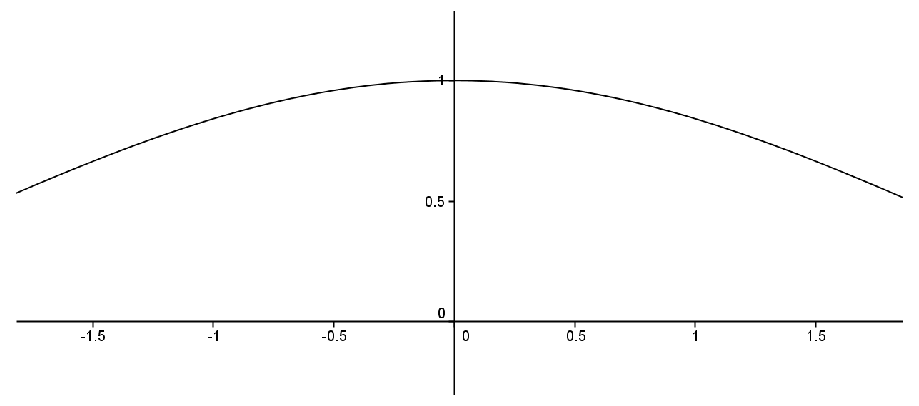
\includegraphics[width=\linewidth]{external/images/SinGraph.png}
		\end{image}%
		From the graph, it appears that \(D(0) =1\) but we must be careful.  \(D(0)\) doesn't even exist!  Somehow we must convey the idea that \(D(x)\) will approach \(1\) as \(x\) approaches \(0\), even though the function is not defined at \(0\).  Cauchy's idea was that the limit of \(D(x)\) would equal \(1\) because we can make \(D(x)\) differ from 1 by as little as we wish~(\hyperlink{x:biblio:jahnke03__histor_analy}{[{\xreffont 6}]}, p. 158).%
		\par
		Karl Weierstrass \index{Weierstrass, Karl} made these ideas precise in his lectures on analysis at the University of Berlin (1859-60) and provided us with our modern formulation.%
		\begin{definition}{}{x:definition:def_limit}%
			\index{limit} We say \(\limit{x}{a}{f(x)} =L\) provided that for each \(\eps>0\), there exists \(\delta>0\) such that if \(0\lt \abs{x-a}\lt \delta\) then \(\abs{f(x)-L}\lt \eps\).%
		\end{definition}
		Before we delve into this, notice that it is very similar to the definition of the continuity of \(f(x)\) at \(x=a\). In fact we can readily see that \(f \text{ is continuous at } x=a \text{ if and only if } \limit{x}{a}{f(x)} = f(a)\).%
		\par
		There are two differences between this definition and the definition of continuity and they are related.  The first is that we replace the value \(f(a)\) with \(L\).  This is because the function may not be defined at \(a\).  In a sense the limiting value \(L\) is the value \(f\) would have \emph{if it were defined and continuous at \(a\).} The second is that we have replaced%
		\begin{equation*}
			\abs{x-a}\lt \delta
		\end{equation*}
		with%
		\begin{equation*}
			0\lt \abs{x-a}\lt \delta\text{.}
		\end{equation*}
		%
		\par
		Again, since \(f\) needn't be defined at \(a\), we will not even consider what happens when \(x=a\). This is the only purpose for this change.%
		\par
		As with the definition of the limit of a sequence, this definition does not determine what \(L\) is, it only verifies that your guess for the value of the limit is correct.%
		\par
		Finally, a few comments on the differences and similiarities between this limit and the limit of a sequence are in order, if for no other reason than because we use the same notation (\(\lim\)) for both.%
		\par
		When we were working with sequences in \hyperref[x:chapter:Convergence]{Chapter~{\xreffont\ref{x:chapter:Convergence}}} and wrote things like \(\limit{n}{\infty}{a_n}\) we were thinking of \(n\) as an integer that got bigger and bigger.  To put that more mathematically, the limit parameter \(n\) was taken from the set of positive integers, or \(n\in \NN\).%
		\par
		For both continuity and the limit of a function we write things like \(\limit{x}{a}{f(x)}\) and think of \(x\) as a variable that gets arbitrarily close to the number \(a\).  Again, to be more mathematical in our language we would say that the limit parameter \(x\) is taken from the \(\ldots\) Well, actually, this is interesting isn't it?  Do we need to take \(x\) from \(\QQ\) or from \(\RR?\) The requirement in both cases is simply that we be able to choose \(x\) arbitrarily close to \(a\). From \hyperref[x:theorem:thm_IrrationalBetweenIrrationals]{Theorem~{\xreffont\ref{x:theorem:thm_IrrationalBetweenIrrationals}}} of \hyperref[x:chapter:NumbersRealRational]{Chapter~{\xreffont\ref{x:chapter:NumbersRealRational}}} we see that this is possible whether \(x\) is rational or not, so it seems either will work.  This leads to the pardoxical sounding conclusion that we do not need a continuum (\(\RR\)) to have continuity.  This seems strange.%
		\par
		Before we look at the above example, let's look at some algebraic examples to see the definition in use.%
		\begin{example}{}{g:example:idp207}%
			Consider the function \(D(x)=\frac{x^2-1}{x-1}\), \(x\neq 1\).  You probably recognize this as the difference quotient used to compute the derivative of \(f(x)=x^2\) at \(x=1\), so we strongly suspect that \(\limit{x}{1}{\frac{x^2-1}{x-1}}=2\).  Just as when we were dealing with limits of sequences, we should be able to use the definition to verify this.  And as before, we will start with some scrapwork.%
			\par
			\terminology{SCRAPWORK}%
			\par
			Let \(\eps>0\).  We wish to find a \(\delta>0\) such that if \(0\lt \abs{x-1}\lt \delta\) then \(\abs{\frac{x^2-1}{x-1}-2}\lt \eps\).  With this in mind, we perform the following calculations%
			\begin{equation*}
				\abs{\frac{x^2-1}{x-1}-2}=\abs{(x+1)-2} = \abs{x-1}\text{.}
			\end{equation*}
			%
			\par
			Now we have a handle on \(\delta\) that will work in the definition and we'll give the formal proof that%
			\begin{equation*}
				\limit{x}{1}{\frac{x^2-1}{x-1}}=2\text{.}
			\end{equation*}
			%
		\end{example}
		\begin{proof}{}{g:proof:idp208}
			Let \(\eps>0\) and let \(\delta=\eps\). If \(0\lt \abs{x-1}\lt \delta\), then%
			\begin{equation*}
				\abs{\frac{x^2-1}{x-1}-2}=\abs{(x+1)-2}=\abs{x-1}\lt \delta=\eps\text{.}\qedhere
			\end{equation*}
			%
		\end{proof}
		As in our previous work with sequences and continuity, notice that the scrapwork is not part of the formal proof (though it was necessary to determine an appropriate \(\delta)\).  Also, notice that \(0\lt \abs{x-1}\) was not really used except to ensure that \(x\neq 1\).%
		\begin{problem}{}{g:problem:idp209}%
			Use the definition of a limit to verify that%
			\begin{equation*}
				\limit{x}{a}{\frac{x^2-a^2}{x-a}}=2a.{}
			\end{equation*}
			%
		\end{problem}
		\begin{problem}{}{g:problem:idp210}%
			Use the definition of a limit to verify each of the following limits.%
			\begin{enumerate}[font=\bfseries,label=(\alph*),ref=\alph*]
				\item{}\(\limit{x}{1}{\frac{x^3-1}{x-1}}=3\)%
				\par\smallskip%
				\noindent\textbf{\blocktitlefont Hint}.\hypertarget{g:hint:idp211}{}\quad{}%
				\begin{align*}
					\abs{\frac{x^3-1}{x-1}-3} \amp = \abs{x^2+x+1-3}\\
					\amp \leq\abs{x^2-1}+\abs{x-1}\\
					\amp =\abs{(x-1+1)^2-1}+\abs{x-1}\\
					\amp =\abs{(x-1)^2+2(x-1)}+\abs{x-1}\\
					\amp \leq\abs{x-1}^2 + 3\abs{x-1}\text{.}
				\end{align*}
				%
				\item{}\(\limit{x}{1}{\frac{\sqrt{x}-1}{x-1}}=1/2\)%
				\par\smallskip%
				\noindent\textbf{\blocktitlefont Hint}.\hypertarget{g:hint:idp212}{}\quad{}%
				\begin{align*}
					\abs{\frac{\sqrt{x}-1}{x-1}-\frac12}\amp = \abs{\frac{1}{\sqrt{x}+1}-\frac12}\\
					\amp =\abs{\frac{2-\left(\sqrt{x}+1\right)}{2\left(\sqrt{x}+1\right)}}\\
					\amp =\abs{\frac{1-x}{2\left(1+\sqrt{x}\right)^2}}\\
					\amp \leq\frac12\abs{x-1}.{}
				\end{align*}
				%
			\end{enumerate}
		\end{problem}
		Let's go back to the original problem: to show that \(\limit{x}{0}{\textstyle\frac{\sin x}{x}}=1\).%
		\par
		While rigorous, our definition of continuity is quite cumbersome. We really need to develop some tools we can use to show continuity rigorously without having to refer directly to the definition. We have already seen in \hyperref[x:theorem:thm_LimDefOfContinuity]{Theorem~{\xreffont\ref{x:theorem:thm_LimDefOfContinuity}}} one way to do this. Here is another. The key is the observation we made after the definition of a limit:%
		\begin{equation*}
			f \text{ is continuous at } x=a \text{ if and only if } \limit{x}{a}{f(x)}=f(a)\text{.}
		\end{equation*}
		%
		\par
		Read another way, we could say that \(\limit{x}{a}{f(x)}=L\) provided that if we redefine \(f(a)=L\) (or define \(f(a)=L\) in the case where \(f(a)\) is not defined) then \(f\) becomes continuous at \(a\). This allows us to use all of the machinery we proved about continuous functions and limits of sequences.%
		\par
		For example, the following corollary to \hyperref[x:theorem:thm_LimDefOfContinuity]{Theorem~{\xreffont\ref{x:theorem:thm_LimDefOfContinuity}}} comes virtually for free once we've made the observation above.%
		\begin{corollary}{}{}{x:corollary:cor_limit-by-sequences}%
			\(\limit{x}{a}{f(x)}=L\) if and only if \(f\) satisfies the following property:%
			\begin{equation*}
				\forall \text{ sequences }  (x_n), x_n\ne a, \text{ if } \limit{n}{\infty}{x_n}=a \text{ then }   \limit{n}{\infty}{f(x_n)}=L. {}
			\end{equation*}
			%
		\end{corollary}
		Armed with this, we can prove the following familiar limit theorems from calculus.%
		\begin{theorem}{}{}{x:theorem:thm_CalcLimits}%
			\index{limit!properties of} Suppose \(\limit{x}{a}{f(x)}=L\) and \(\limit{x}{a}{g(x)}=M\), then%
			\begin{enumerate}[label=(\alph*)]
				\item{}\(\displaystyle \limit{x}{a}{\left(f(x)+g(x)\right)}=L+M\)%
				\item{}\(\displaystyle \limit{x}{a}{\left(f(x)\cdot g(x)\right)}=L\cdot M\)%
				\item{}\(\limit{x}{a}{\left(\frac{f(x)}{g(x)}\right)}=L/M\) provided \(M\ne0\) and \(g(x)\ne{}0\), for \(x\) sufficiently close to a (but not equal to \(a\)).%
			\end{enumerate}
			%
		\end{theorem}
		We will prove part (a) to give you a feel for this and let you prove parts (b) and (c).%
		\begin{proof}{}{g:proof:idp213}
			Let \(\left(x_n\right)\) be a sequence such that \(x_n\ne
			a\) and \(\limit{n}{\infty}{x_n}=a\).  Since \(\limit{x}{a}{f(x)} = L\) and \(\limit{x}{a}{g(x)} =
			M\) we see that \(\limit{n}{\infty}{f(x_n)} = L\) and \(\limit{n}{\infty}{g(x_n)} = M\).  By \hyperref[x:theorem:thm_SumOfSequences]{Theorem~{\xreffont\ref{x:theorem:thm_SumOfSequences}}} of \hyperref[x:chapter:Convergence]{Chapter~{\xreffont\ref{x:chapter:Convergence}}}, we have \(\limit{n}{\infty}{f(x_n)+g(x_n)}=L+M\).  Since \(\left\{x_n\right\}\) was an arbitrary sequence with \(x_n\ne a\) and \(\limit{n}{\infty}{x_n} = a\) we have%
			\begin{equation*}
				\limit{x}{a}{f(x)+g(x)} = L+M\text{.}\qedhere
			\end{equation*}
			%
		\end{proof}
		\begin{problem}{}{g:problem:idp214}%
			\index{limit!properties of}\index{limit!verify limit laws from calculus} Prove parts (b) and (c) of \hyperref[x:theorem:thm_CalcLimits]{Theorem~{\xreffont\ref{x:theorem:thm_CalcLimits}}}.%
		\end{problem}
		More in line with our current needs, we have a reformulation of the Squeeze Theorem.%
		\begin{theorem}{}{}{x:theorem:thm_SqueezeTheoremFunctions}%
			\alert{Squeeze Theorem for functions}%
			\par
			\index{Squeeze Theorem!for functions} Suppose \(f(x)\le g(x) \le h(x)\), for \(x\) sufficiently close to \(a\) (but not equal to \(a\)). If \(\limit{x}{a}{f(x)}=L=\limit{x}{a}{h(x)}\), then \(\limit{x}{a}{g(x)}=L\) also.%
		\end{theorem}
		\begin{problem}{}{g:problem:idp215}%
			\index{Squeeze Theorem!for functions} Prove \hyperref[x:theorem:thm_SqueezeTheoremFunctions]{Theorem~{\xreffont\ref{x:theorem:thm_SqueezeTheoremFunctions}}}.%
			\par\smallskip%
			\noindent\textbf{\blocktitlefont Hint}.\hypertarget{g:hint:idp216}{}\quad{}Use \hyperref[x:theorem:thm_SqueezeTheorem]{Theorem~{\xreffont\ref{x:theorem:thm_SqueezeTheorem}}}, the Squeeze Theorem for sequences from \hyperref[x:chapter:Convergence]{Chapter~{\xreffont\ref{x:chapter:Convergence}}}.%
		\end{problem}
		Returning to \(\limit{x}{0}{\frac{\sin x}{x}}\) we'll see that the Squeeze Theorem is just what we need.  First notice that since \(D(x)=\sin x/x\) is an even function, we only need to focus on \(x>0\) in our inequalities.  Consider the unit circle.%
		\begin{image}{0.2}{0.6}{0.2}%
			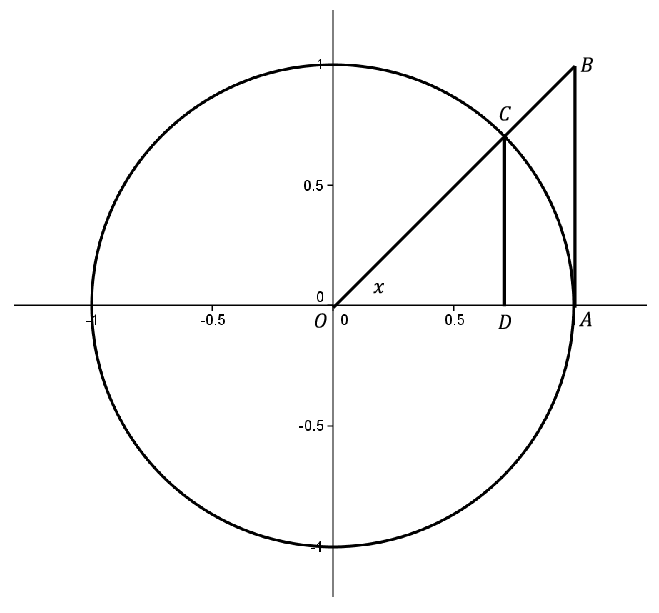
\includegraphics[width=\linewidth]{external/images/UnitCircle.png}
		\end{image}%
		\begin{problem}{}{g:problem:idp217}%
			Use the fact that%
			\begin{equation*}
				\text{ area } (\Delta OAC)\lt \text{ area } (\text{ sector } OAC)\lt \text{ area } (\Delta OAB)
			\end{equation*}
			to show that if \(0\lt x\lt \pi/2\), then \(\cos x\lt
			\sin x/x\lt 1\).  Use the fact that all of these functions are even to extend the inequality for \(-\pi/2\lt x\lt
			0\) and use the Squeeze Theorem to show \(\limit{x}{0}{\textstyle\frac{\sin x}{x}}=1\).%
		\end{problem}
	\end{sectionptx}
	%
	%
	\typeout{************************************************}
	\typeout{Section 9.4 The Derivative, An Afterthought}
	\typeout{************************************************}
	%
	\begin{sectionptx}{The Derivative, An Afterthought}{}{The Derivative, An Afterthought}{}{}{x:section:Continuity-DerivativeAfterthought}
		No, the derivative isn't really an afterthought.  Along with the integral it is, in fact, one of the most powerful and useful mathematical objects ever devised and we've been working very hard to provide a solid, rigorous foundation for it.  In that sense it is a primary focus of our investigations.%
		\par
		On the other hand, now that we have built up all of the machinery we need to define and explore the concept of the derivative it will appear rather pedestrian alongside ideas like the convergence of power series, Fourier series, and the bizarre properties of \(\QQ\) and \(\RR\).%
		\par
		You spent an entire semester learning about the properties of the derivative and how to use them to explore the properties of functions so we will not repeat that effort here.  Instead we will define it formally in terms of the ideas and techniques we've developed thus far.%
		\begin{definition}{The Derivative.}{x:definition:def_derivative}%
			\index{differentiation!definition of the derivative}%
			Given a function \(f(x)\) defined on an interval \((a,b)\) we define%
			\begin{equation*}
				f^\prime(x) = \limit{h}{0}{\frac{f(x+h)-f(x)}{h}}.{}
			\end{equation*}
			%
		\end{definition}
		There are a few fairly obvious facts about this definition which are nevertheless worth noticing explicitly:%
		\par
		%
		\begin{enumerate}
			\item{}The derivative is \emph{defined at a point.} If it is defined at every point in an interval \((a,b)\) then we say that the derivative exists at every point on the interval.%
			\item{}Since it is defined at a point it is at least theoretically possible for a function to be differentiable at a single point in its entire domain.%
			\item{}Since it is defined as a limit and not all limits exist, functions are not necessarily differentiable.%
			\item{}Since it is defined as a limit, \hyperref[x:corollary:cor_limit-by-sequences]{Corollary~{\xreffont\ref{x:corollary:cor_limit-by-sequences}}} applies. That is, \(f^\prime(x)\) exists if and only if \(\forall \text{ sequences } (h_n),\, h_n\ne 0\), if \(\limit{n}{\infty}{h_n}=0\) then%
			\begin{equation*}
				f^\prime{(x)} =
				\limit{n}{\infty}{\frac{f(x+h_n)-f(x)}{h_n}} \text{.}
			\end{equation*}
			Since \(\limit{n}{\infty}{h_n}=0\) this could also be written as%
			\begin{equation*}
				f^\prime{(x)} = \limit{h_n}{0}{\frac{f(x+h_n)-f(x)}{h_n}}\text{.}
			\end{equation*}
			%
		\end{enumerate}
		%
		\begin{theorem}{}{}{x:theorem:thm_DiffImpCont}%
			\index{continuity!implied by differentiability}%
			\index{differentiation!differentiability implies continuity}%
			\alert{Differentiability Implies Continuity}%
			\par
			If \(f\) is differentiable at a point \(c\) then \(f\) is continuous at \(c\) as well.%
		\end{theorem}
		\begin{problem}{}{g:problem:idp218}%
			Prove \hyperref[x:theorem:thm_DiffImpCont]{Theorem~{\xreffont\ref{x:theorem:thm_DiffImpCont}}}%
		\end{problem}
		As we mentioned, the derivative is an extraordinarily useful mathematical tool but it is not our intention to learn to \emph{use} it here.  Our purpose here is to define it rigorously (done) and to show that our formal definition does in fact recover the useful properties you came to know and love in your calculus course.%
		\par
		The first such property is known as Fermat's Theorem.%
		\begin{theorem}{Fermat's Theorem.}{}{x:theorem:thm_FermatsTheorem}%
			\index{Fermat's Theorem}%
			Suppose \(f\) is differentiable in some interval \((a,b)\) containing \(c\).  If \(f(c)\ge f(x)\) for every \(x\) in \((a,b)\), then \(f^\prime(c)=0\).%
		\end{theorem}
		\begin{proof}{}{g:proof:idp219}
			Since \(f^\prime(c)\) exists we know that if \(\left(h_n\right)_{n=1}^\infty\) converges to zero then the sequence \(a_n = \frac{f\left(c+h_n\right)-f(c)}{h_n}\) converges to \(f^\prime(c)\).  The proof consists of showing that \(f^\prime(c)\leq 0\) \emph{and} that \(f^\prime(c)\geq
			0\) from which we conclude that \(f^\prime(c)= 0\).  We will only show the first part.  The second is left as an exercise.%
			\par
			\emph{Claim:} \(f^\prime(c)\leq 0\).%
			\par
			Let \(n_0\) be sufficiently large that \(\frac{1}{n_0}\lt b-c\) and take \(\left(h_n\right)=\left(\frac{1}{n}\right)_{n=n_0}^\infty\). Then \(f\left(c+\frac1n\right)-f(c) \leq 0\) and \(\frac1n>0\), so that%
			\begin{equation*}
				\frac{f\left(c+h_n\right)-f(c)}{h_n}\leq 0, \ \ \forall n=n_0, n_0+1, \ldots
			\end{equation*}
			%
			\par
			Therefore \(f^\prime(c) = \limit{h_n}{0}{\frac{f\left(c+h_n\right)-f(c)}{h_n}} \leq 0\) also.%
		\end{proof}
		\begin{problem}{}{g:problem:idp220}%
			\index{Fermat's Theorem!if \(f(a)\) is a maximum then \(f^\prime(a)=0\)} Show that \(f^\prime(c) \geq 0\) and conclude that \(f^\prime(c) =0\).%
		\end{problem}
		\begin{problem}{}{g:problem:idp221}%
			\index{Fermat's Theorem!if \(f(a)\) is a minimum then \(f^\prime(a)=0\)} Show that if \(f(c) \leq f(x)\) for all \(x\) in some interval \((a,b)\) then \(f^\prime(c) =0\) too.%
		\end{problem}
		Many of the most important properties of the derivative follow from what is called the Mean Value Theorem (\terminology{MVT}) which we now state.%
		\begin{theorem}{}{}{x:theorem:thm_MVT}%
			\terminology{The Mean Value Theorem}%
			\par
			\index{Mean Value Theorem, the} Suppose \(f^\prime\) exists for every \(x\in(a,b)\) and \(f\) is continuous on \([a,b]\). Then there is a real number \(c\in(a,b)\) such that%
			\begin{equation*}
				f^\prime(c)=\frac{f(b)-f(a)}{b-a}.{}
			\end{equation*}
			%
		\end{theorem}
		However, it would be difficult to prove the MVT right now. So we will first state and prove Rolle's Theorem, which can be seen as a special case of the MVT. The proof of the MVT will then follow easily.%
		\par
		Michel Rolle first stated the following theorem in 1691. Given this date and the nature of the theorem it would be reasonable to suppose that Rolle was one of the early developers of calculus but this is not so. In fact, Rolle was disdainful of both Newton \index{Newton, Isaac} and Leibniz's\index{Leibniz, Gottfried Wilhelm} versions of calculus, once deriding them as a collection of ``ingenious fallacies.'' It is a bit ironic that his theorem is so fundamental to the modern development of the calculus he ridiculed.%
		\begin{theorem}{}{}{x:theorem:thm_Rolle_s_Theorem}%
			\index{Rolle's Theorem}%
			\terminology{Rolle's Theorem}%
			\par
			Suppose \(f^\prime\) exists for every \(x\in(a,b)\), \(f\) is continuous on \([a,b]\), and%
			\begin{equation*}
				f(a)=f(b)\text{.}
			\end{equation*}
			%
			\par
			Then there is a real number \(c\in(a,b)\) such that%
			\begin{equation*}
				f^\prime(c)=0\text{.}
			\end{equation*}
			%
		\end{theorem}
		\begin{proof}{}{g:proof:idp222}
			\begin{aside}{}{g:aside:idp223}%
				Any proof that relies on the Extreme Value Theorem is not complete until the EVT has been proved. We'll get to this in \hyperref[x:chapter:IVTandEVT]{Chapter~{\xreffont\ref{x:chapter:IVTandEVT}}}.%
			\end{aside}
			Since \(f\) is continuous on \([a,b]\) we see, by the Extreme Value Theorem,\index{Extreme Value Theorem (EVT)!Rolle's Theorem, and} that \(f\) has both a maximum and a minimum on \([a,b]\). Denote the maximum by \(M\) and the minimum by \(m\). There are several cases:%
			\begin{descriptionlist}
				\begin{dlimedium}{Case 1:}{g:li:idp224}%
					\(f(a)=f(b)=M=m\). In this case \(f(x)\) is constant (why?). Therefore \(f^\prime(x)=0\) for every \(x\in(a,b)\).%
				\end{dlimedium}%
				\begin{dlimedium}{Case 2:}{g:li:idp225}%
					\(f(a)=f(b)=M\neq m\). In this case there is a real number \(c\in(a,b)\) such that \(f(c)\) is a local minimum. By Fermat's Theorem, \(f^\prime(c)=0\).%
				\end{dlimedium}%
				\begin{dlimedium}{Case 3:}{g:li:idp226}%
					\(f(a)=f(b)=m\neq M\). In this case there is a real number \(c\in(a,b)\) such that \(f(c)\) is a local maximum. By Fermat's Theorem, \(f^\prime(c)=0\).%
				\end{dlimedium}%
				\begin{dlimedium}{Case 4:}{g:li:idp227}%
					\(f(a)=f(b)\) is neither a maximum nor a minimum. In this case there is a real number \(c_1\in(a,b)\) such that \(f(c_1)\) is a local maximum, and a real number \(c_2\in(a,b)\) such that \(f(c_2)\) is a local minimum. By Fermat's Theorem, \(f^\prime(c_1)=f^\prime(c_2)=0\).%
				\end{dlimedium}%
			\end{descriptionlist}
			%
		\end{proof}
		With Rolle's Theorem in hand we can prove the MVT which is really a corollary to Rolle's Theorem or, more precisely, it is a generalization of Rolle's Theorem. To prove it we only need to find the right function to apply Rolle's Theorem to. The following figure shows a function, \(f(x)\), cut by a secant line, \(L(x)\), from \((a, f(a))\) to \((b,f(b))\).%
		\begin{image}{0.22}{0.56}{0.22}%
			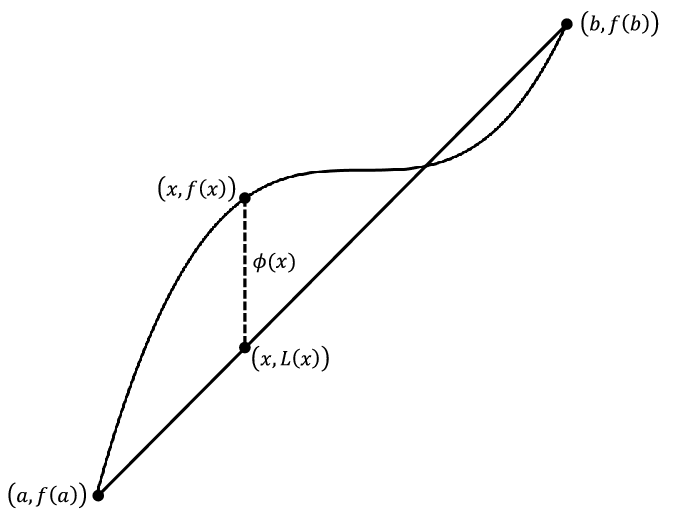
\includegraphics[width=\linewidth]{external/images/MVT.png}
		\end{image}%
		The vertical difference from \(f(x)\) to the secant line, indicated by \(\phi(x)\) in the figure should do the trick. You take it from there.%
		\begin{problem}{}{g:problem:idp228}%
			\index{Mean Value Theorem, the} Prove the Mean Value Theorem.%
		\end{problem}
		The Mean Value Theorem is extraordinarily useful. Almost all of the properties of the derivative that you used in calculus follow more or less easily from it. For example the following is true.%
		\begin{corollary}{}{}{x:corollary:cor_PosDerivIncFunc1}%
			If \(f^\prime(x) > 0\) for every \(x\) in the interval \((a,b)\) then for every \(c,d\in(a,b)\) where \(d>c\) we have%
			\begin{equation*}
				f(d) > f(c) \text{.}
			\end{equation*}
			%
			\par
			That is, \(f\) is increasing on \((a,b)\).%
		\end{corollary}
		\begin{proof}{}{g:proof:idp229}
			Suppose \(c\) and \(d\) are as described in the corollary. Then by the Mean Value Theorem there is some number, say \(\alpha\in(c,d)\subseteq(a,b)\) such that%
			\begin{equation*}
				f^\prime(\alpha)=\frac{f(d)-f(c)}{d-c}\text{.}
			\end{equation*}
			%
			\par
			Since \(f^\prime(\alpha)>0\) and \(d-c>0\) we have \(f(d)-f(c)>0\), or \(f(d)>f(c)\).%
		\end{proof}
		\begin{problem}{}{g:problem:idp230}%
			\index{differentiation!if \(f^\prime\lt 0\) on an interval then \(f\) is decreasing} Show that if \(f^\prime(x) \lt 0\) for every \(x\) in the interval \((a,b)\) then \(f\) is decreasing on \((a,b)\).%
		\end{problem}
		\begin{corollary}{}{}{x:corollary:cor_PosDerivIncFunc2}%
			Suppose \(f\) is differentiable on some interval \((a,b)\), \(f^\prime\) is continuous on \((a,b)\), and that \(f^\prime(c)>0\) for some \(c\in (a,b)\). Then there is an interval, \(I\subset (a,b)\), containing \(c\) such that for every \(x,
			y\) in \(I\) where \(x\ge y\), \(f(x)\ge f(y)\).%
		\end{corollary}
		\begin{problem}{}{g:problem:idp231}%
			\index{differentiation!\(f^\prime(a)>0\) implies \(f\) is increasing nearby} Prove \hyperref[x:corollary:cor_PosDerivIncFunc2]{Corollary~{\xreffont\ref{x:corollary:cor_PosDerivIncFunc2}}}.%
		\end{problem}
		\begin{problem}{}{g:problem:idp232}%
			\index{differentiation!\(f^\prime(a)\lt 0\) implies \(f\) is decreasing nearby} Show that if \(f\) is differentiable on some interval \((a,b)\) and that \(f^\prime(c)\lt 0\) for some \(c\in (a,b)\) then there is an interval, \(I\subset (a,b)\), containing \(c\) such that for every \(x, y\) in \(I\) where \(x\le y\), \(f(x)\le f(y)\).%
		\end{problem}
	\end{sectionptx}
	%
	%
	\typeout{************************************************}
	\typeout{Section 9.5 Additional Problems}
	\typeout{************************************************}
	%
	\begin{sectionptx}{Additional Problems}{}{Additional Problems}{}{}{x:section:Continuity-AddProb}
		\begin{problem}{}{g:problem:idp233}%
			Use the definition of continuity to prove that the constant function \(g(x)=c\) is continuous at any point \(a\).%
		\end{problem}
		\begin{problem}{}{g:problem:idp234}%
			\begin{enumerate}[font=\bfseries,label=(\alph*),ref=\alph*]
				\item{}Use the definition of continuity to prove that \(\ln x\) is continuous at \(1\).%
				\par\smallskip%
				\noindent\textbf{\blocktitlefont Hint}.\hypertarget{g:hint:idp235}{}\quad{}You may want to use the fact \(\abs{\ln x}\lt \eps\,\Leftrightarrow-\eps\lt \ln x\lt \eps\) to find a \(\delta\).%
				\item{}Use part (a) to prove that \(\ln x\) is continuous at any positive real number \(a\).%
				\par\smallskip%
				\noindent\textbf{\blocktitlefont Hint}.\hypertarget{g:hint:idp236}{}\quad{}\(\ln(x)=\ln(x/a)+\ln(a)\). This is a combination of functions which are continuous at \(a\). Be sure to explain how you know that \(\ln(x/a)\) is continuous at \(a\).%
			\end{enumerate}
		\end{problem}
		\begin{problem}{}{g:problem:idp237}%
			\index{continuity!formal definition of discontinuity} Write a formal definition of the statement \(f\) is not continuous at \(a\), and use it to prove that the function \(f(x)= \begin{cases}x\amp \text{ if } x\neq 1\\ 0\amp \text{ if } x=1 \end{cases}\) is not continuous at \(a=1\).%
		\end{problem}
	\end{sectionptx}
\end{chapterptx}
%
%